Wasser hat den Brechungsindex $n=1.333=\frac43$.
Ein kugelförmiger Wassertropfen vom Radius $r=1$ fokusiert Licht in 
einem Brennpunkt (siehe auch Abbildung~\ref{10000060:fig}).
Wie weit von der Kugeloberfläche ist der Brennpunkt entfernt?

\begin{figure}[h]
\centering
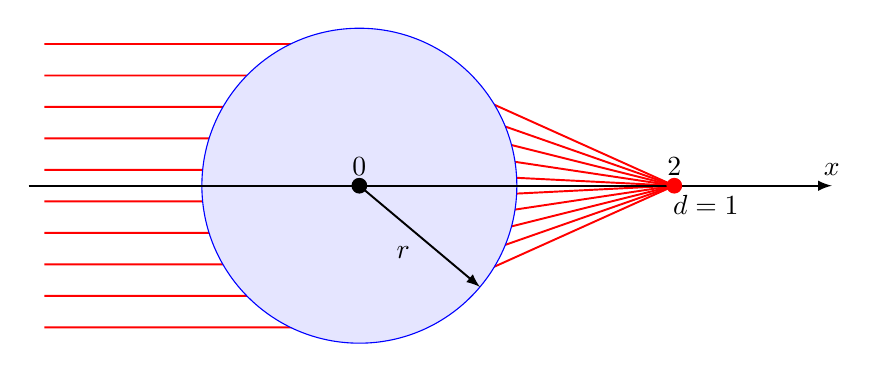
\begin{tikzpicture}[>=latex,scale=2]
\foreach \x in {0.1,0.3,...,0.9}{
\draw[line width=0.7pt,color=red] (-2,{\x})--(0,{\x})--(2,0);
\draw[line width=0.7pt,color=red] (-2,{-\x})--(0,{-\x})--(2,0);
}
\fill[color=blue!10] (0,0) circle[radius=1];
\draw[color=blue] (0,0) circle[radius=1];
\draw[->,line width=0.7pt] (-2.1,0)--(3,0) coordinate[label={$x$}];
\draw[->,line width=0.7pt] (0,0)--({cos(-40)},{sin(-40)});
\node at ({0.5*cos(-40)},{0.5*sin(-40)}) [below left] {$r$};
\fill (0,0) circle[radius=0.05];
\fill[color=red] (2,0) circle[radius=0.05];
\node at (0,0) [above] {$0$};
\ifthenelse{\boolean{loesungen}}{
\node at (2,0) [above] {$2$};
\node at (2.2,0) [below] {$d=1$};
}{}
\end{tikzpicture}
\caption{Fokusierende Wirkung eines kugelförmigen Wassertropfens
\label{10000060:fig}}
\end{figure}

\begin{hinweis}
Rechnen Sie in paraxialer Näherung.
\end{hinweis}

\thema{Matrixoptik}

\begin{loesung}
Die Transfermatrizen der beiden Flächen sind
\begin{align*}
T_l
&=
B(1,n,r)
=
B(1,{\textstyle \frac43},1)
=
\begin{pmatrix} 1&0\\\frac34-1&\frac34 \end{pmatrix}
=
\begin{pmatrix} 1&0\\-\frac14&\frac34 \end{pmatrix}
\\
\text{und}\qquad
T_r
&=
B(n,1,-r)
=
B({\textstyle \frac43},1,-1)
=
\begin{pmatrix} 1&0\\-\frac43+1&\frac43 \end{pmatrix}
=
\begin{pmatrix} 1&0\\-\frac13&\frac43 \end{pmatrix}.
\end{align*}
Die gekrümmten Flächen sind $2r=2$ voneinander entfernt, ein Lichstrahl
entwickelt sich mit der Matrix 
\[
T_2
=
\begin{pmatrix}1&2\\0&1\end{pmatrix}.
\]
Die Transfermatrix des Wassertropfens ist daher
\[
T
=
T_rT_2T_l
=
\begin{pmatrix} 1&0\\-\frac13&\frac43 \end{pmatrix}
\begin{pmatrix}1&2\\0&1\end{pmatrix}
\begin{pmatrix} 1&0\\-\frac14&\frac34 \end{pmatrix}
=
\begin{pmatrix} 1&0\\-\frac13&\frac43 \end{pmatrix}
\begin{pmatrix} \phantom{-}\frac12 & \frac32 \\ -\frac14 & \frac34 \end{pmatrix}
=
\begin{pmatrix}
\phantom{-}\frac12 & \frac32 \\
-\frac12 & \frac12
\end{pmatrix}.
\]

Der Brennpunkt befinde sich in der Entfernung $d$ von der Kugeloberfläche.
Die Matrx $T_d$ beschreibt die Entwicklung des Strahls bis zu diesem Punkt.
Dies ergibt die Matrix
\[
T_dT
=
\begin{pmatrix}
1&d\\0&1
\end{pmatrix}
\begin{pmatrix}
\phantom{-}\frac12 & \frac32 \\
-\frac12 & \frac12
\end{pmatrix}
=
\begin{pmatrix}
\frac12(1-d) & \frac12(3+d) \\
-\frac12 & \frac12
\end{pmatrix}.
\]

Ein einfallender Strahl wird durch den Standardbasisvektor $e_1$ beschrieben,
dessen zweite Komponenten verschwindet.
Der ausfallende Strahl ist daher 
\[
T_dTe_1
=
\begin{pmatrix}
\frac12(1-d) & \frac12(3+d) \\
-\frac12 & \frac12
\end{pmatrix}
\begin{pmatrix}1\\0\end{pmatrix}
=
\begin{pmatrix}
\frac12(1-d) \\
-\frac12 \\
\end{pmatrix}
\]
Gesucht ist der Wert $d$, für den die erste Komponente verschwindet.
Dies ist offenbar der Punkt mit $d=1$.
\end{loesung}

\begin{bewertung}
Transfermatrix für beide gekrümmten Flächen ({\bf B}) 2 Punkte,
Transfermatrix für Distanz ({\bf D}) 1 Punkt,
Matrizenmultiplikation ({\bf M}) 1 Punkt,
Bedingung für Brennpunkt ({\bf F}) 1 Punkt,
Position des Brennpunktes ({\bf P}) 1 Punkt.
\end{bewertung}



